\section{Ablauf chemischer Reaktionen}

\subsection{Thermochemie}
\subsubsection{Enthalpie}
Beschreibt den Wärmeinhalt eines Systems, Prinzip Energieminimum:
$$\boxed{\Delta H_R = H_{Produkte} - H_{Edukte}} $$
\begin{tabular}{l l}
	$\Delta H_R < 0 \text{ \textbf{exotherm}, Energie wird frei}$ & $\Delta H_R > 0 \text{ \textbf{endotherm}, Energie wird aufgenommen}$ \\
	$\text{[H]} =\frac{J}{mol}$ & \\
\end{tabular}
\subsubsection{Entropie}
Beschreibt verschiedene Anordnungsmöglichkeiten von Teilchen in einem System,\break Prinzip Energiemaximum:
$$\boxed{\Delta S_R = S_{Produkte} - S_{Edukte}} $$
\begin{tabular}{l l}
	$\Delta S_R < 0 \text{  \textbf{Unordnung nimmt ab} z.B. wenn Gase zu Flüssigkeit reagieren}$ &  \\
	$\Delta S_R > 0 \text{  \textbf{Unordnung nimmt zu} z.B. wenn ein Feststoff zu Gas wird}$     &  \\
	$\text{[S]}=\frac{J}{mol \cdot K}$                                                            & \\
\end{tabular}

\subsubsection{Freie Enthalpie}
Gibbs-Helmholtz-Gleichung definiert, ob eine Reaktion bei konstanter Temperatur und konstantem Druck freiwillig (spontan) verlauft:
$$\boxed{\Delta G = \Delta H - T \cdot \Delta S} $$
\begin{tabular}{l l}
	$\Delta G < 0 \text{  \textbf{freiwillig} Exergon}$    &  \\
	$\Delta G > 0 \text{  \textbf{unfreiwillig} Endergon}$ &  \\
	$\text{[G]}=\frac{J}{mol}$                             & \\
\end{tabular}

\subsection{Reaktionsgeschwindigkeit}

$$ \boxed{\text{RGT-Faustregel:}\pm T=\pm 10^{\circ}C \rightarrow  \text{um Faktor 2 erhöhen oder senken (in d, h, min)}}$$

Chemische Reaktionen benötigen eine Aktivierungsenergie. \newline 
Diese sagt aus, wie schnell die Reaktion passiert.
Exotherme Reaktionen verlaufen nach anfänglicher Aktivierung oft freiwillig.

\subsubsection{Katalysatoren}
\label{Reaktionsgeschw}
\begin{minipage}{0.2\linewidth}
	% \vspace*{0pt}
	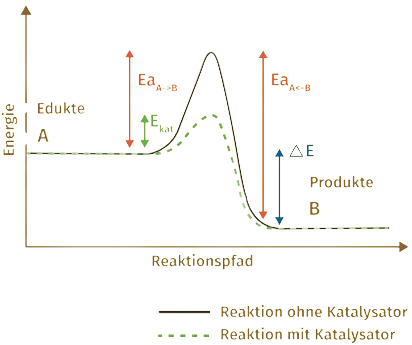
\includegraphics[width=\linewidth]{images/Katalysator_1.png}
\end{minipage}
\hfill
\begin{minipage}{0.65\linewidth}
	\begin{itemize}
		\item Katalysator = Stoff nimmt an Reaktion teil, wird nicht verbraucht 
		\item Beschleunigt Reaktion: $E_{AKat} \ll E_{ANorm}$
		\item $\Delta$ G sowie $\Delta H_R$ bleiben gleich
		\item Selektiv (wirkt nicht mit allen Stoffen)
	\end{itemize}
\end{minipage}

